\documentclass[10pt,showpacs,showkeys,twocolumn]{revtex4-1}
%%%%%%%%%%%%%%%%%%%%%%%%%%%%%%%%%%%%%%%%%%%%%%%%%%%%%%%%%%%%%%%%%%%%%%%%
% \usepackage[T1]{fontspec}
\usepackage{bm}
\usepackage{amssymb}
\usepackage{amsmath}
\usepackage{graphicx}
\usepackage{multirow}
\usepackage{MnSymbol}
\usepackage{wasysym} 
\usepackage{stmaryrd}
\usepackage[outline]{contour}
\usepackage[dvipsnames]{xcolor}
\usepackage{float}

\definecolor{olive}{RGB}{182,187,37}
\usepackage[mathlines]{lineno}% Enable numbering of text and display math
%\linenumbers\relax % Commence numbering lines

\begin{document}

\title[General scaling rule for the ionization of biological molecules]{
General scaling rule for the ionization of biological molecules \\ by 
highly charged ions}
\author{A. M. P. Mendez, C. C. Montanari, J. E. Miraglia}
\affiliation{Instituto de Astronom\'{\i}a y F\'{\i}sica del Espacio 
(CONICET-UBA), \\ Buenos Aires, Argentina.}

\date{}% It is always \today, today,

\begin{abstract}
In the present work, we investigate scaling rules for the ionization 
cross sections of multicharged ions on molecules of biological interest. 
The cross sections are obtained using a methodology presented in 
[Mendez \textit{et al.} J. Phys B (2020)], which considers distorted-wave 
calculations for atomic targets combined with a molecular stoichiometric 
model. We examine ions with nuclear charges $Z$ from $+1$ to $+8$ 
impacting on five nucleobases --adenine, cytosine, guanine, thymine, 
uracil--, tetrahydrofuran, pyrimidine, and water. We propose a scaling 
with the ion charge, which is valid in the intermediate to high energy 
range, i.e., 0.2-5 MeV/amu for oxygen impact. We extend our work to a 
universal scaling for any ion and molecule, merging the forty 
ion-molecule systems analyzed here into a single band. Furthermore, our 
model proved to be valid for other molecules too.  
\end{abstract}

\keywords{ionization, scaling, molecules, charged-ions, DNA, 
multicharged ions}
\pacs{34.50Gb, 34.80Gs, 34.80Dp}

\maketitle
%\ioptwocol
\linenumbers

The ionization of biological molecules by multicharged ions has gained 
increasing interest due to medical and environmental 
implementations~\cite{PhysMed}, which includes medical 
treatments~\cite{Mohamad2017,Solov2009,Denifl2011} and contaminant 
recognition in biological materials~\cite{water,ferrazdias}. 
Many semiempirical \citep{vera_prl2013} and theoretical efforts are 
currently being undertaken~\cite{MendezJPB20,Quinto20,ludde2019,ludde2018,
ludde2016,Champion2012} to get reliable values for the ionization cross 
sections of these molecular systems. 

In recent work~\cite{MendezJPB20}, we combined the continuum 
distorted-wave calculations (CDW) for atoms and the simple 
stoichiometric model (SSM), also known as the Bragg sum rule, to 
approximate the ionization cross sections of complex molecular targets 
by charged ions. The CDW-SSM approximation showed consistent results 
for over a hundred of ion-molecule systems. As expected, in the high 
energy range (i.e., above 5 MeV/amu), the ionization cross sections of
the molecular systems follow the $Z^2$ dependence predicted by the 
first Born approximation. However, at intermediate energies, the 
dependence with $Z$ is not straightforward since non-perturbative 
models are mandatory.

This letter intends to give a follow up of our previous work by 
proposing a scaling rule for the ionization cross sections of complex 
molecules with the ion charge $Z$, which is valid at intermediate 
energies. In general, scaling rules are used as first-order 
approximations in experimental measurements and multipurpose codes. 
Furthermore, we explore the generality of our scaling rule by inspecting 
various other ion-target systems.

We have found in the literature two scaling rules applicable at 
intermediate impact energy range. The scaling rule suggested by Janev 
and Presnyakov~\cite{janev1980} depends linearly with ion charge $Z$,
considering $\sigma/Z$ versus $E/Z$ to be the \textit{natural} reduced 
form of the ionization cross section $\sigma$ and the incident ion 
energy $E$. More recently, Montenegro and co-workers~\cite{dubois13,
montenegro_pra13} proposed an alternative scaling by taking into account 
that the cross section is a function of $Z^2/E$. Their scaling, given by 
\begin{equation}
    \sigma/Z^{\alpha}=f(E/Z^{2-\alpha}),
    \label{Montenegro}
\end{equation}
keeps the $Z^2/E$ relationship for any value of the parameter $\alpha$. 
In Ref.~\cite{dubois13}, the authors propose $\alpha=4/3$ for ionization 
of He and H$_2$ by differently charged ions. 

Combining our recent CDW-SSM results~\cite{MendezJPB20} and 
Eq.~(\ref{Montenegro}), we propose here a $Z$-scaling and implement it 
for forty collisional systems. The ion-molecule systems are composed of 
eight targets: the DNA and RNA nucleobases --adenine, cytosine, guanine, 
thymine, uracil--, tetrahydrofuran (THF), pyrimidine, and water; and 
five ion species: H$^+$, He$^{+2}$, Be$^{+4}$, C$^{+6}$, and O$^{+8}$. 
We considered these systems as a benchmark for the present scaling. 

We found that the parameter $\alpha$ from Eq.~(\ref{Montenegro}) that 
fits the CDW-SSM scaled cross sections for all the ions is $\alpha=1.2$. 
The validity of the theoretical scaling with the ion charge is evident
in Fig.~\ref{fig:zreduced}, where the CDW-SSM curves lay one over the 
other. Our theoretical results are valid for impact energies around and 
above the maximum of the cross sections, which corresponds to an impact
energy range from 50 keV for H$^+$ to 250 keV/amu for O$^{+8}$. 

The scaling was tested with the experimental data available for 
ionization by the impact of differently charged ions \cite{itoh2013,
iriki2011,wolff2014,wang2016,tribedi2019,agnihotri2012,agnihotri2013,
Luna2007,Rudd86,Rudd85,Luna_Li_water,DalCappello2009,Tribedi_O_water}, 
and also by electron impact at sufficiently high velocity 
\cite{rahman2016,bug2017,wolf2019,fuss2009}. As can be noted, most of 
the data in Fig.~\ref{fig:zreduced} confirm the present scaling, even 
for O$^{+8}$ in water~\cite{Tribedi_O_water}. However, the data of 
uracil by swift C, O, and F ions in \cite{agnihotri2012,agnihotri2013} 
are too low compared with our CDW-SSM results, but also as compared 
with Itoh \textit{et al.} data \cite{itoh2013}, and with the CTMC 
calculations by Sarkadi~\cite{sarkadi2016}. The data for Li$^{+3}$ in 
water from Ref.~\cite{Luna_Li_water} also spreads out from the present 
theoretical curves for $E<600$ keV/amu.

The good results obtained in the scaling with the ion charge challenged 
us to look for a more general scaling rule that could predict values 
for ionization cross sections of any ion in any molecule. To that end, 
we resorted to the number of active electrons in each atom $n_e$ 
proposed in \cite{MendezJPB20}, and combined it with the $Z$-scaling 
displayed in Fig.~\ref{fig:zreduced}.


\begin{figure*}[!htb]
\centering
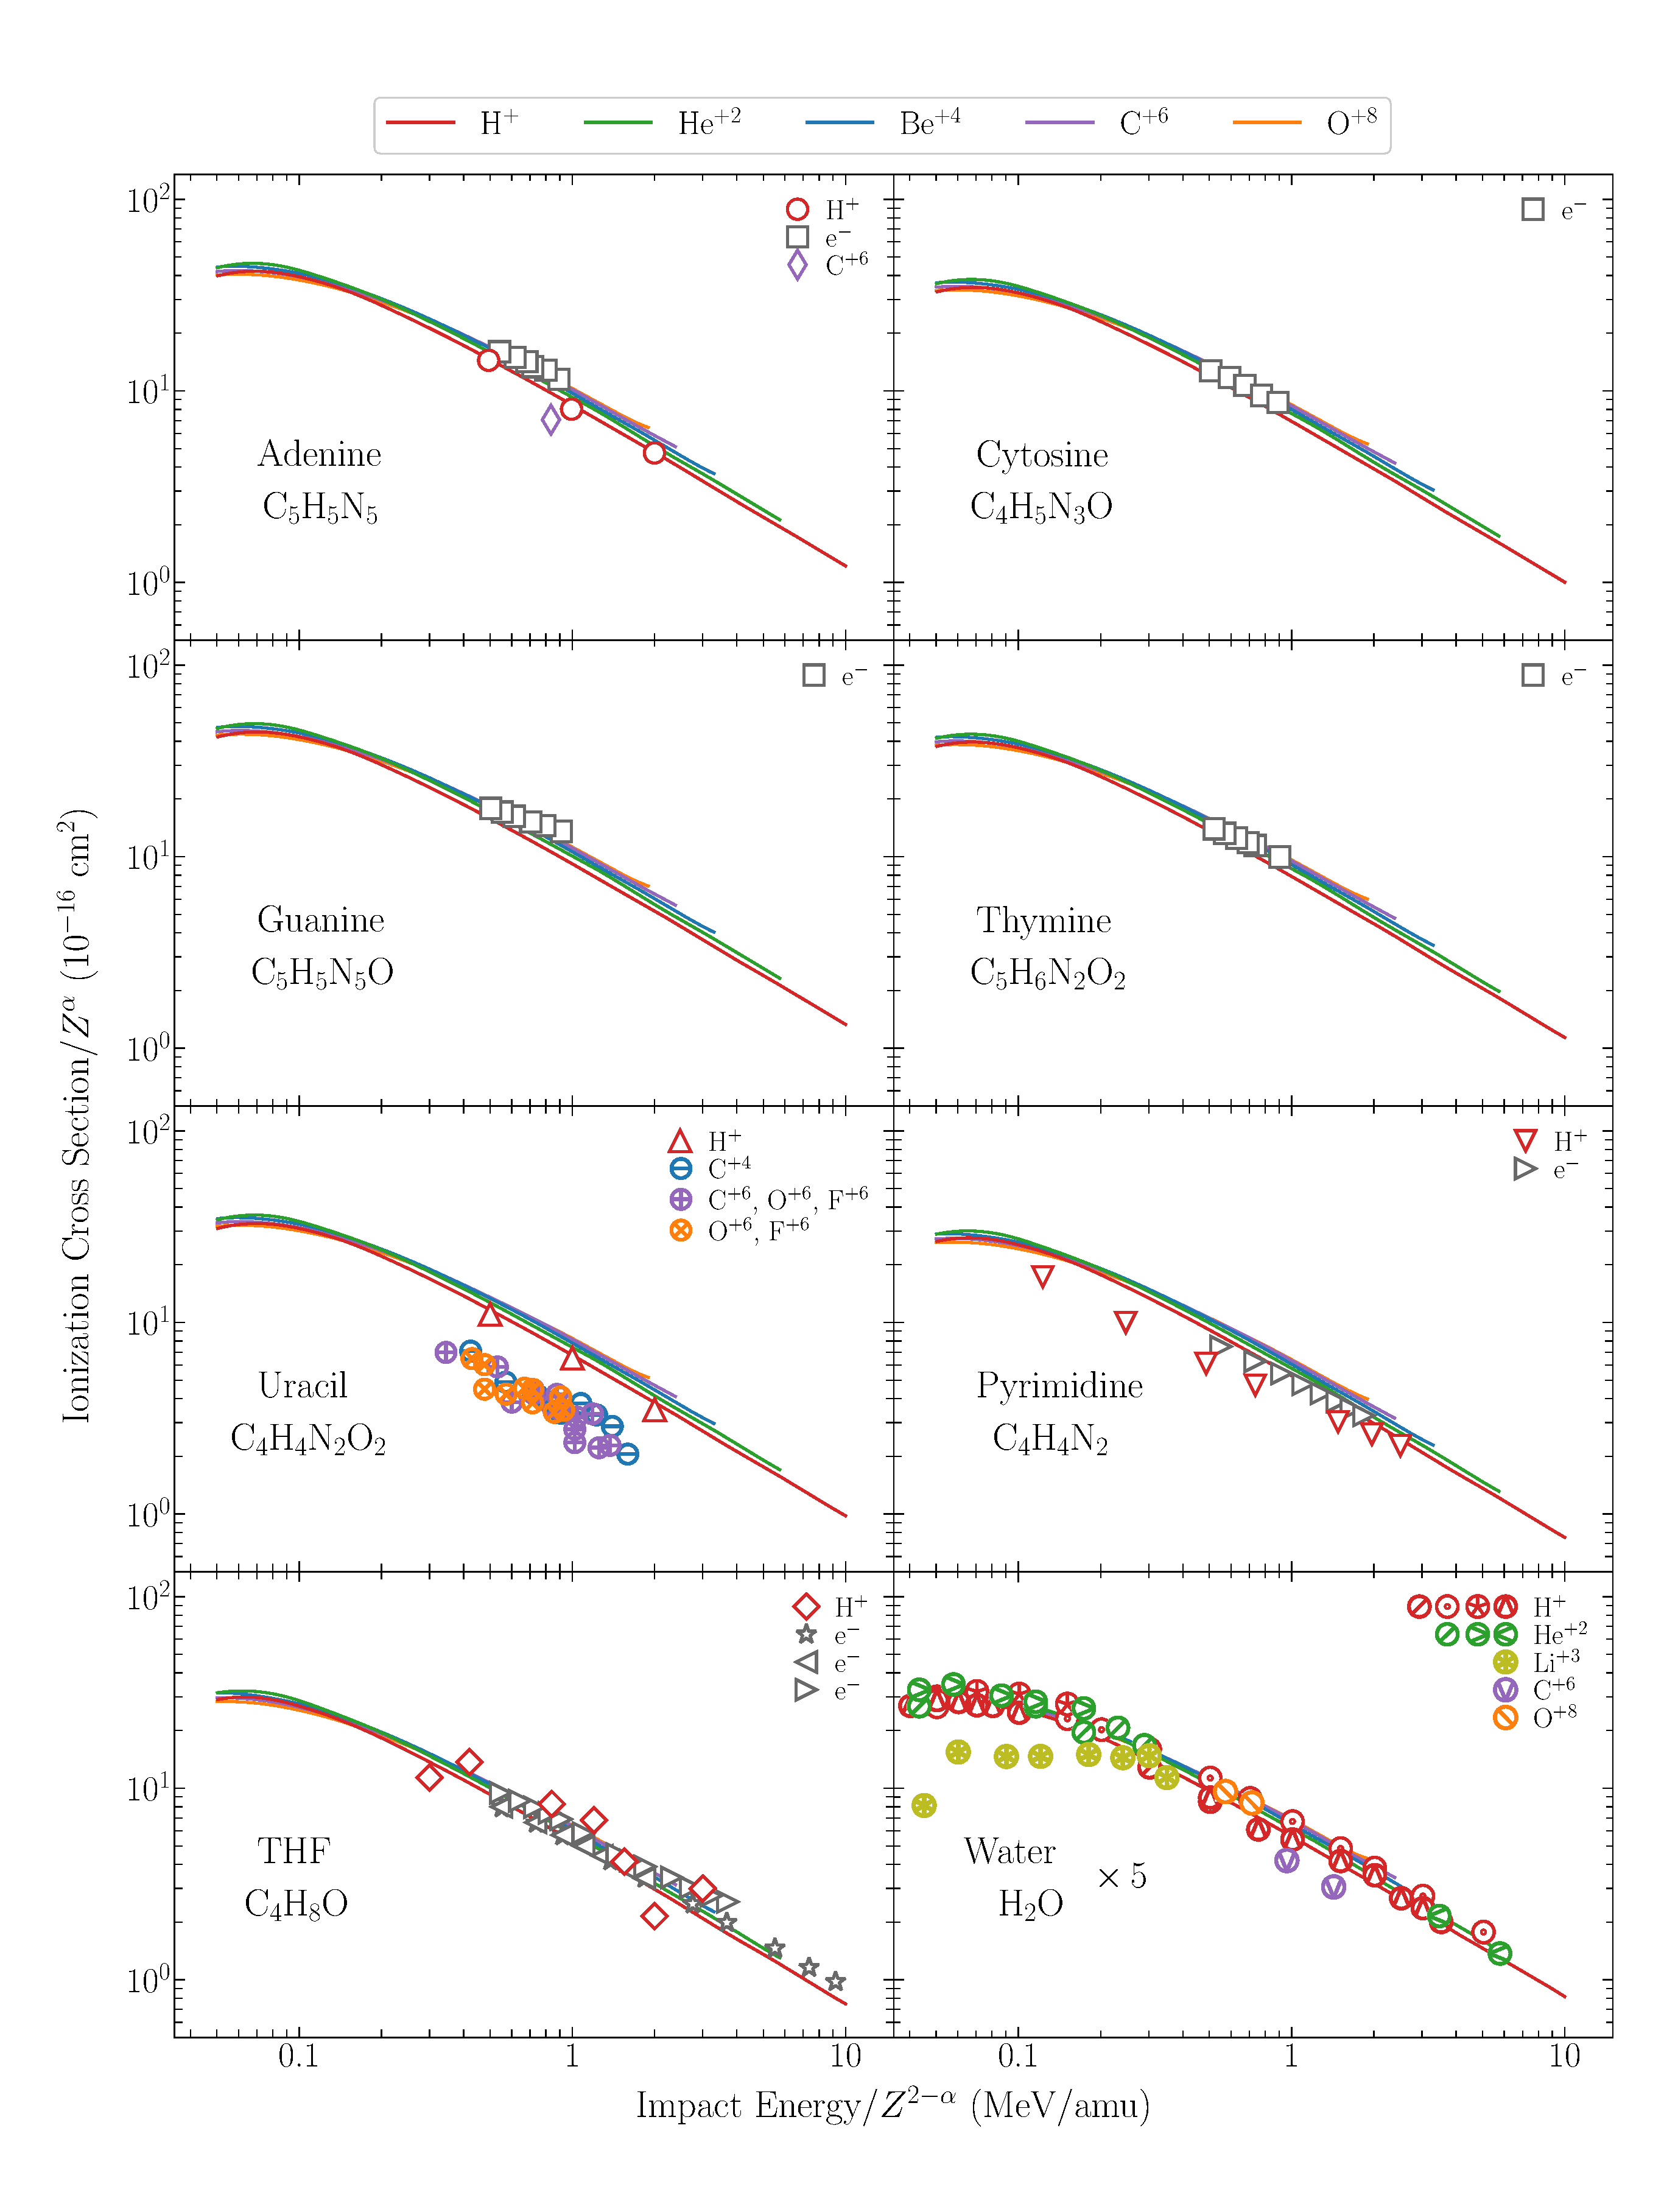
\includegraphics[width=0.9\textwidth]{zscale_alpha.eps}
\caption{(Color online) Scaled ionization cross section $\sigma/Z^{\alpha}$ 
as a function of ion impact energy $E/Z^{2-\alpha}$ with $\alpha=1.2$. 
Colors are associated with the incident ion labeled on top of the figure. 
Curves: present CDW-SSM theoretical results. Symbols: experimental 
impact of \mbox{\LARGE$\color{red}\circ$} H$^+$~\cite{iriki2011} and
{\fontsize{11}{20}$\color{Purple}\pmb{\lozenge}$} C$^{+6}$ 
\cite{tribedi2019} on adenine;
H$^+$ on {\fontsize{11}{20}$\color{red}\pmb{\triangle}$} uracil~\cite{itoh2013}, 
{\fontsize{11}{20}$\color{NavyBlue}\pmb{\ominus}$} C$^{+4}$, 
{\fontsize{11}{20}$\color{Purple}\pmb{\oplus}$} C$^{+6}$, O$^{+6}$, F$^{+6}$, and 
{\fontsize{11}{20}$\color{BurntOrange}\pmb{\otimes}$} O$^{+8}$, 
F$^{+8}$ on uracil~\cite{agnihotri2012,agnihotri2013};
H$^+$ on {\fontsize{11}{20}$\color{red}\pmb{\triangledown}$} 
pyrimidine~\cite{wolff2014}, and 
{\fontsize{10}{20}$\color{red}\pmb{\meddiamond}$} THF~\cite{wang2016};
% water
\mbox{\fontsize{11}{20}$\color{red}\pmb{\odot}$}~\cite{Luna2007}, 
{\fontsize{11}{20}\color{red}$\pmb{\logof}$}~\cite{Rudd86}, 
{\fontsize{11}{20}\color{red}$\pmb{\varowedge}$}~\cite{pRudd85}, 
{\fontsize{11}{20}\color{red}$\pmb{\varoslash}$}~\cite{toburen80} H$^+$,
{\fontsize{11}{20}\color{ForestGreen}$\pmb{\varolessthan}$}~\cite{Ohsawa05},
{\fontsize{11}{20}\color{ForestGreen}$\pmb{\varogreaterthan}$}~\cite{Rudd85},
{\fontsize{11}{20}\color{ForestGreen}$\pmb{\varoslash}$}~\cite{toburen80} He$^{+2}$,
{\fontsize{11}{20}\color{Purple}$\pmb{\ovee}$}~C$^{+6}$ \cite{DalCappello2009,Bhattacharjee17}, and 
{\fontsize{11}{20}\color{BurntOrange}$\pmb{\obslash}$}
O$^{+8}$ \cite{Tribedi_O_water} on water.
Markers~$\square$~\cite{rahman2016}, 
$\rhd$~\cite{bug2017}, 
$\lhd$~\cite{wolf2019}, and 
$\medstar$~\cite{fuss2009} correspond to electron impact ionization with 
the equi-velocity conversion.}
\label{fig:zreduced}
\end{figure*} 

The CDW ionization cross sections $\sigma^{\mathrm{CDW}}$ of atomic H, 
C, N, O targets scale as $\sigma_e=\sigma^{\mathrm{CDW}}/n_e$ with $n_e$ 
being $1$ for H, $4$ for C, N, and O, i.e.,
\begin{equation}
 \frac{\sigma_{\mathrm{H}}^{\mathrm{CDW}}}{1}\sim
 \frac{\sigma_{\mathrm{C}}^{\mathrm{CDW}}}{4}\sim
 \frac{\sigma_{\mathrm{N}}^{\mathrm{CDW}}}{4}\sim
 \frac{\sigma_{\mathrm{O}}^{\mathrm{CDW}}}{4}
\end{equation}
The SSM leads to the molecular numbers of active electrons included in 
Table \ref{nn}.

\contourlength{0.03em}
\contournumber{30}

\begin{table}[t]
\begin{center}
\begin{tabular}{|ll|ll|ll|}
\hline
 Molecule & $n_e$ & Molecule          & $n_e$ & Molecule          & $n_e$ \\
\hline
 H$_2$O   & 6  & CO$_2$               & 12 & C$_4$H$_5$N$_3$O     & 37   \\ 
 N$_2$    & 8  & C$_4$H$_8$O          & 28 & C$_5$H$_6$N$_2$O$_2$ & 42   \\ 
 O$_2$    & 8  & C$_4$H$_4$N$_2$      & 28 & C$_5$H$_5$N$_5$      & 45   \\ 
 CH$_4$   & 8  & C$_4$H$_4$N$_2$O$_2$ & 36 & C$_5$H$_5$N$_5$O     & 49   \\ 
 \hline
\end{tabular}
\caption{Number of active electrons per target at intermediate to high 
energies obtained from the CDW calculations~\cite{MendezJPB20}.}
\label{nn}
\end{center}
\end{table}

\begin{figure*}[!t]%[h]
\centering
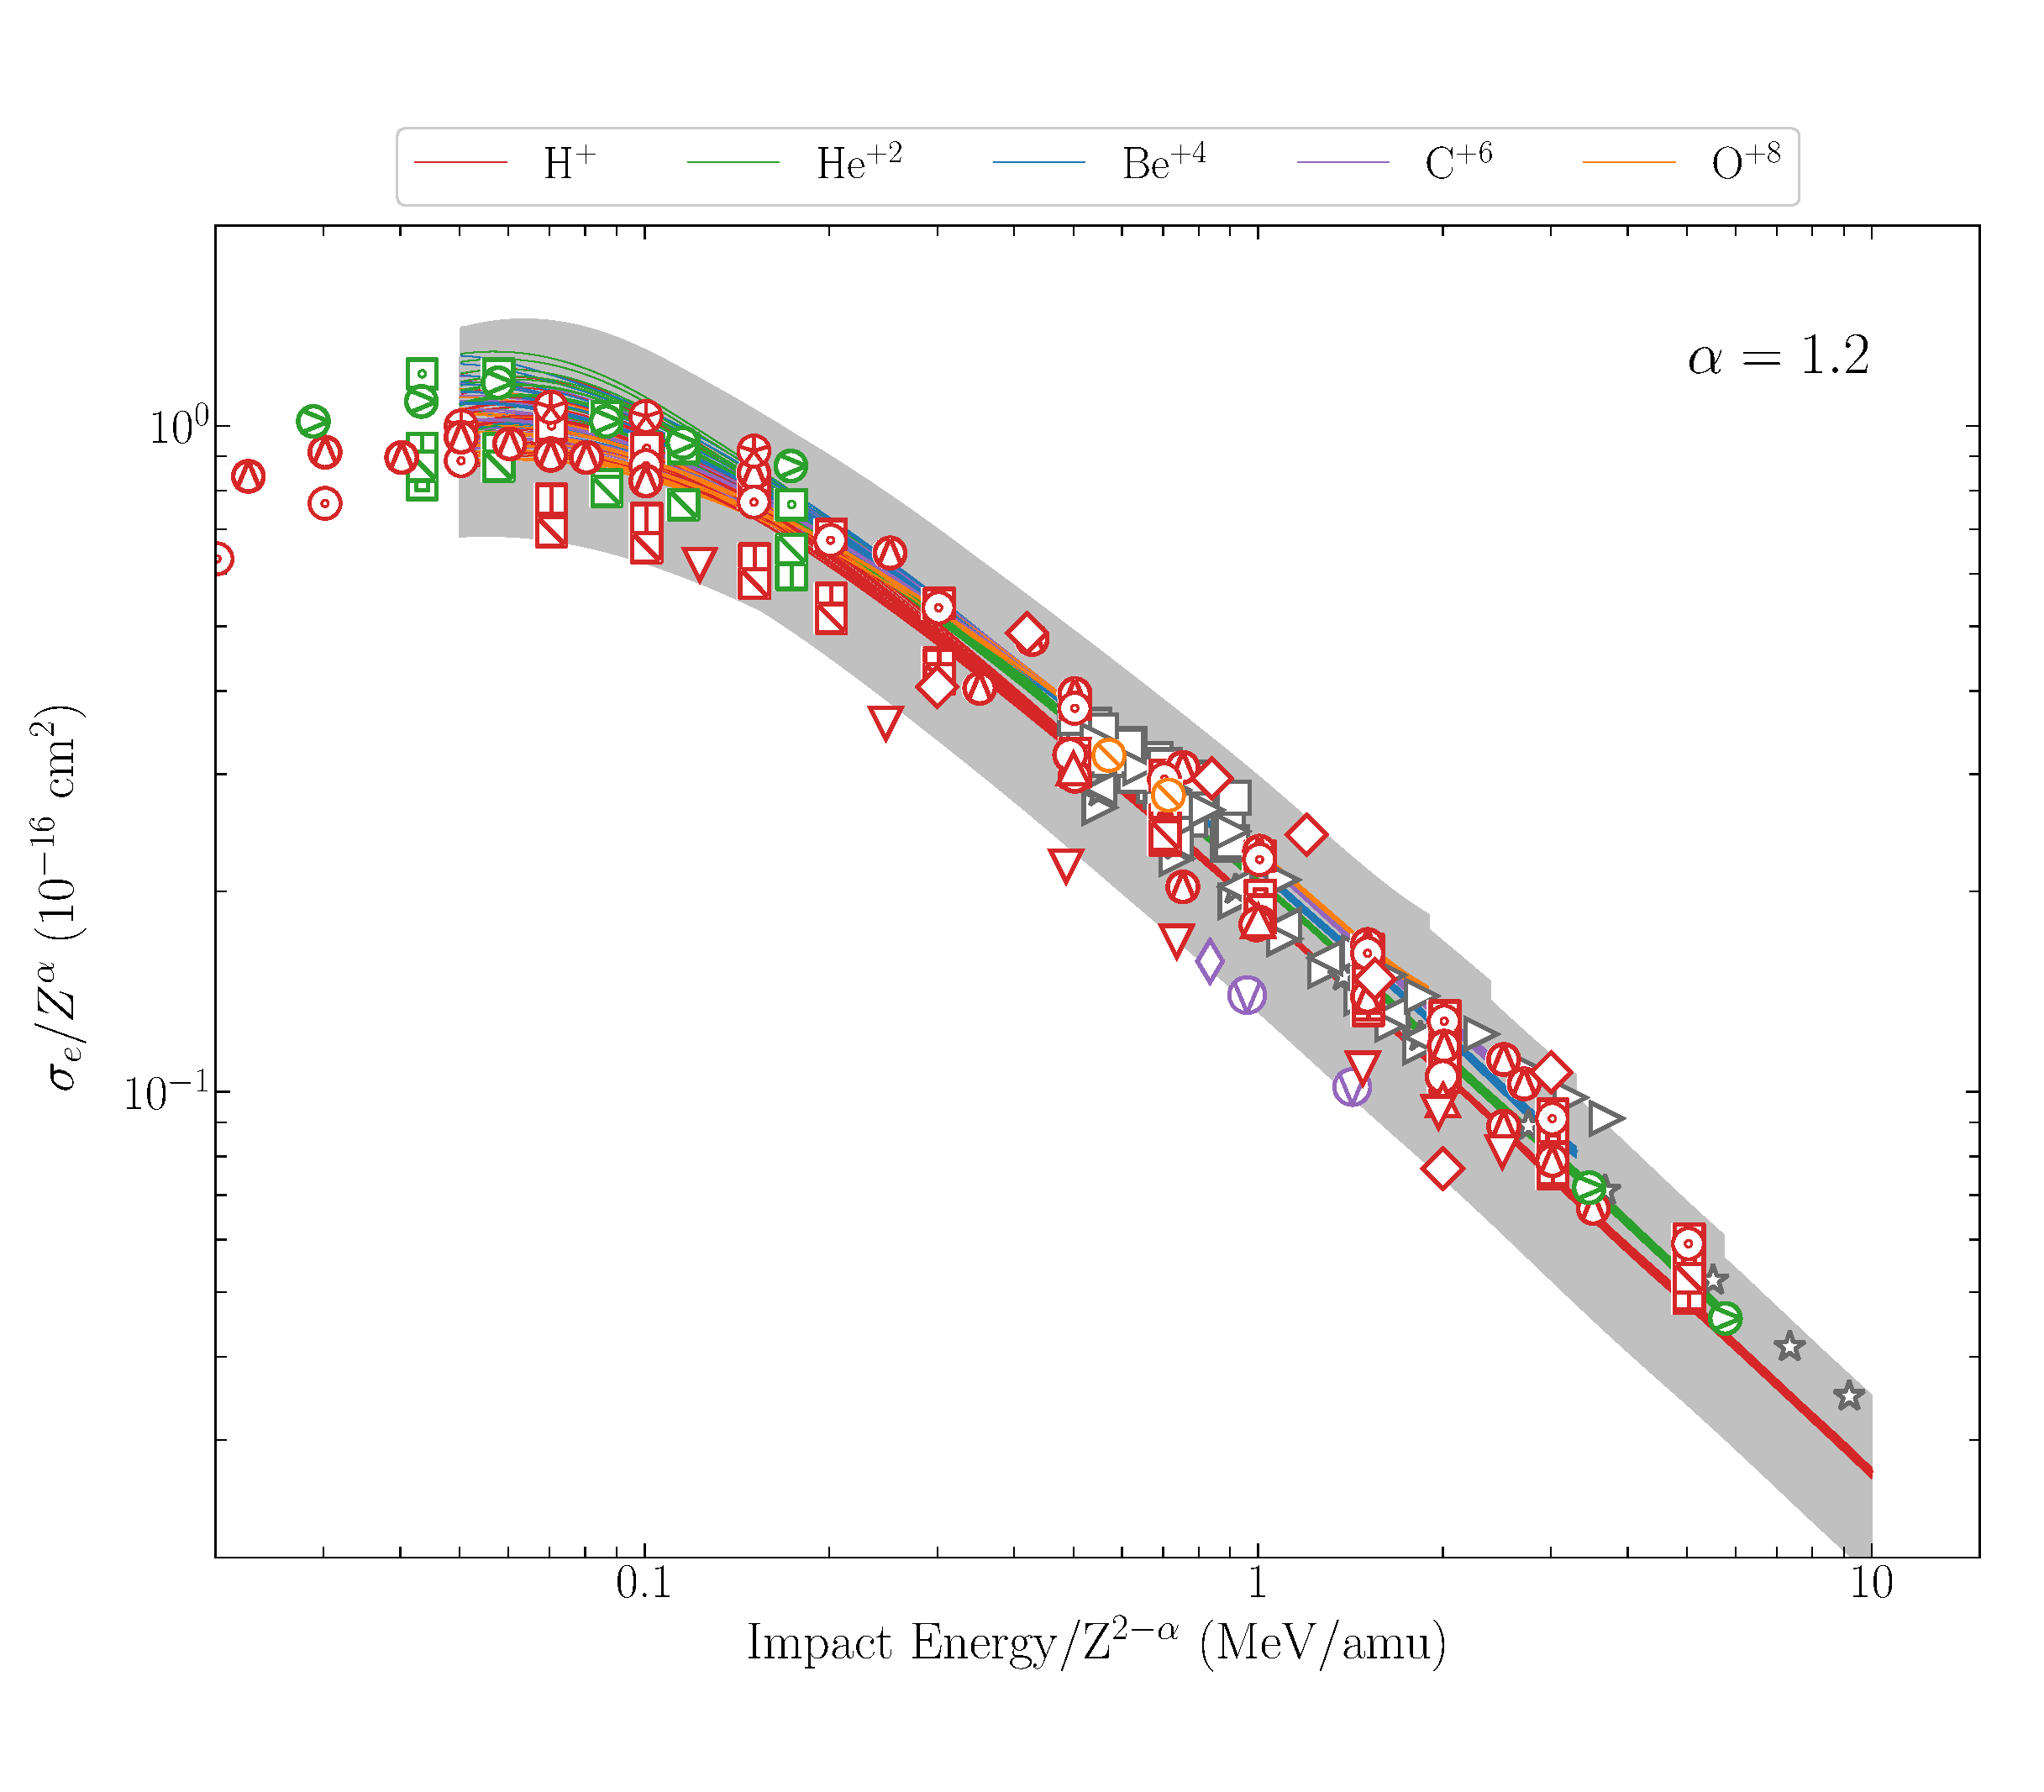
\includegraphics[width=0.7\textwidth]{zmol_werror.eps}
\caption{(Color online) Universal scaling with the ions charge $Z$ and 
the number of active electrons in the molecule $n_e$ given by Eq. 
(\ref{u-scaling}) with $\alpha=1.2$. Curves: present CDW-SSM theoretical 
results. Symbols: experimental impact of H$^+$ on 
\mbox{\LARGE$\color{red}\circ$} adenine~\cite{iriki2011}, 
{\fontsize{11}{20}$\color{red}\pmb{\triangle}$} uracil~\cite{itoh2013}, 
{\fontsize{11}{20}$\color{red}\pmb{\triangledown}$} pyrimidine~\cite{wolff2014} and 
{\fontsize{10}{20}$\color{red}\pmb{\meddiamond}$} THF~\cite{wang2016};
{\fontsize{11}{20}$\color{Purple}\pmb{\lozenge}$} C$^{+6}$ on adenine \cite{tribedi2019};
\mbox{\fontsize{11}{20}$\color{red}\pmb{\odot}$}~\cite{Luna2007}, 
{\fontsize{11}{20}\color{red}$\pmb{\logof}$}~\cite{Rudd86}, 
{\fontsize{11}{20}\color{red}$\pmb{\varowedge}$}~\cite{pRudd85}, 
{\fontsize{11}{20}\color{red}$\pmb{\varoslash}$}~\cite{toburen80} H$^+$,
{\fontsize{11}{20}\color{ForestGreen}$\pmb{\varolessthan}$}~\cite{Ohsawa05},
{\fontsize{11}{20}\color{ForestGreen}$\pmb{\varogreaterthan}$}~\cite{Rudd85},
{\fontsize{11}{20}\color{ForestGreen}$\pmb{\varoslash}$}~\cite{toburen80} He$^{+2}$,
{\fontsize{11}{20}\color{Purple}$\pmb{\ovee}$}~C$^{+6}$ \cite{DalCappello2009,Bhattacharjee17}, and 
{\fontsize{11}{20}\color{BurntOrange}$\pmb{\obslash}$}
O$^{+8}$ \cite{Tribedi_O_water} on water.
H$^{+}$ impact on 
{\fontsize{11}{20}${\color{red}\pmb{\boxast}}$}~N$_2$, 
{\fontsize{11}{20}${\color{red}\pmb{\boxbox}}$}~O$_2$, 
{\fontsize{11}{20}${\color{red}\pmb{\boxbar}}$}~CO, 
{\fontsize{11}{20}${\color{red}\pmb{\boxbslash}}$}~CO$_2$, and
{\fontsize{11}{20}${\color{red}\pmb{\boxdot}}$}~CH$_4$; 
and He$^{+2}$ impact on 
{\fontsize{11}{20}${\color{ForestGreen}\pmb{\boxast}}$}~N$_2$,
{\fontsize{11}{20}${\color{ForestGreen}\pmb{\boxbox}}$}~O$_2$, 
{\fontsize{11}{20}${\color{ForestGreen}\pmb{\boxbar}}$}~CO, 
{\fontsize{11}{20}${\color{ForestGreen}\pmb{\boxbslash}}$}~CO$_2$, and
{\fontsize{11}{20}${\color{ForestGreen}\pmb{\boxdot}}$} 
CH$_4$~\cite{Rudd85,Rudd1983}, 
{\fontsize{11}{20}${\color{red}\pmb{\varowedge}}$}~H$^{+}$ on 
CH$_4$~\cite{Luna2019}; 
and electron impact on $\rhd$~pyrimidine~\cite{bug2017}, and $\lhd$, 
$\medstar$~\cite{wolf2019,fuss2009} THF.}
\label{fig:zalpha}
\end{figure*} 
 
The universal scaling we propose here is expressed as $\sigma_U$ as a 
function of $E/Z^{2-\alpha}$, with
 \begin{equation}
     \sigma_U=\frac{\sigma_e}{Z^{\alpha}}=\frac{\sigma/n_e}{Z^{\alpha}}\,,
     \label{u-scaling}
 \end{equation}
$\sigma$ is the ionization cross section for the molecular target, 
$\alpha=1.2$ and $n_e$ is the number of active electrons per molecule 
given in Table \ref{nn}. In Fig.~\ref{fig:zalpha}, we test the universal 
scaling of Eq.~(\ref{u-scaling}) for all the theoretical and 
experimental values displayed in Fig. \ref{fig:zreduced}. We also 
included a gray area representing the 30\% deviation of our theoretical 
curves. As can be noted, the universal scaling works very well. All the 
curves and data lays in a narrow band valid for any charged ion (scaled 
with Z) in any molecule (scaled with the number of active electrons). 
We decided not to include in this figure the data for uracil from 
Refs.~\cite{agnihotri2012,agnihotri2013}, and for Li$^{+3}$ on 
water~\cite{Luna_Li_water}. The discussion about these experimental 
values exceeds the present work. %is open for future work.

In principle, the \textit{universal} scaling should be valid for 
different ion--molecule combinations. We proved this statement by 
including in Fig.~\ref{fig:zalpha} the measurements by 
Rudd~\textit{et al.} \cite{Rudd85,Rudd1983} for H$^{+}$ and He$^{+2}$ 
in N$_2$, O$_2$, CH$_4$, CO and CO$_2$, and the recent values by 
Luna~\textit{et al.} \cite{Luna2019} for H$^{+}$ in CH$_4$. 

The good agreement shown in Fig.~\ref{fig:zalpha} summaries the main 
result of this work, and holds the validity of our universal scaling. 
Although the theoretical CDW-SSM results are valid for energies above 
the maximum of the cross sections, the scaling of the experimental data 
extends to lower impact energies, as can be noted in 
Fig.~\ref{fig:zalpha}. The importance of scaling rules lays in their 
predictive capability. New measurements for other ions and molecules 
are expected to reinforce the present proposal. 

%%%%%%%%%%%%%%%%%%%%%%%%%%%%%%%%%%%%%%%%%%%%%%%%%%%%%%%%%%%%%%%%%%%%%%%%
\section{Conclusions}
In this letter, we present a scaling for the ionization cross sections 
of highly charged ions in biological targets. The scaling rule states 
the cross sections divided by $Z^{\alpha}$ as a function of the reduced 
impact energy $E/Z^{2-\alpha}$, with $\alpha=1.2$. The scaling was 
obtained by means of the CDW-SSM calculations for five different charged 
ions in eight targets and tested with the available experimental data. 
A universal scaling rule  is also proposed, which reduced the cross 
sections with the number of active electrons of the molecule. The 
universal scaling proved to be valid for a large number of experimental 
data.

%%%%%%%%%%%%%%%%%%%%%%%%%%%%%%%%%%%%%%%%%%%%%%%%%%%%%%%%%%%%%%%%%%%%%%%%

\begin{thebibliography}{}

% intro --------------------------------------------------------
\bibitem{PhysMed} 
T. Liamsuwan and H. Nikjoo, 
Phys. Med. Biol. \textbf{58}  641--672 (2013).

\bibitem{Mohamad2017}
O. Mohamad, B. J. Sishc, J. Saha, A. Pompos, A. Rahimi, M. D. Story, 
A. J. Davis, D. N. Kim, 
Cancers \textbf{9}, 66 (2017).

\bibitem{Solov2009}
A. V. Solov'yov, E. Surdutovich, E. Scifoni, I. Mishustin, and 
W. Greiner, 
Phys. Rev. E \textbf{79}, 011909 (2009);
% https://link.aps.org/doi/10.1103/PhysRevE.79.011909

\bibitem{Denifl2011}
Denifl S., Märk T.D., Scheier P. 
% The Role of Secondary Electrons in Radiation Damage. 
% In Radiation Damage in Biomolecular Systems. Biological and Medical Physics, Biomedical Engineering. 
Eds: Garc\'ia G\'omez-Tejedor G., Fuss M. 
Springer, Dordrecht (2012) 

\bibitem{water} 
N. A. Gafur, M.  Sakakibara, S. Sano, K. A. Sera, 
% \textit{Case Study of Heavy Metal Pollution in Water of Bone River by Artisanal Small-Scale Gold Mine Activities in Eastern Part of Gorontalo, Indonesia}, 
Water \textbf{10}, 1507 (2018); doi:10.3390/w10111507.

\bibitem{ferrazdias} 
D. Benedetti, E. Nunes, M. Sarmento, C. Porto, C. E. Iochims dos Santos, 
J. Ferraz Dias, J. da Silva,
% \textit{Genetic damage in soybean workers exposed to pesticides: Evaluation with the comet and buccal micronucleus cytome assays},
Mutation Research/Genetic Toxicology and Environmental Mutagenesis,
Volume 752, 28-33 (2013);
% https://doi.org/10.1016/j.mrgentox.2013.01.001.

\bibitem{vera_prl2013} 
P. de Vera, R. Garcia-Molina,I. Abril, and A. V. Solov’yov, 
Phys. Rev. Lett.  110, 148104 (2013).

% our ---------------------------------------------------------
\bibitem{MendezJPB20}
A. M. P. Mendez, C. C. Montanari, and J. E. Miraglia, 
J. Phys. B: At. Mol. Opt. Phys.  \textbf{53}, 055201 (2020).

% others -----------------------------------------------
\bibitem{Quinto20} 
M. A. Quinto, J. M. Monti, C. A. Tachino, P. F. Weck, O. A. Foj\'on, 
C. Champion, R. D. Rivarola, 
% \textit{The physics of irradiation of biological matter by ion beams}, 
Rad. Phys. Chem. \textbf{167}, 108337 (2020);
% https://doi.org/10.1016/j.radphyschem.2019.05.027.

\bibitem{ludde2019}
H. J. L\"udde,  M. Horbatsch and T. Kirchner, 
J. Phys. B: At. Mol. Opt. Phys. \textbf{52}, 195203 (2019).

\bibitem{ludde2018}
H. J. L\"udde, M. Horbatsch and T. Kirchner, 
Eur. Phys. J. B \textbf{91}, 99 (2018).

\bibitem{ludde2016}
H. J. L\"udde, A. Achenbach, T. Kalkbrenner, H.-C. Jankowiak and T. Kirchner,
Eur. Phys. J. D \textbf{70}, 82 (2016).

\bibitem{Champion2012} 
C. Champion, M. E. Galassi, O. Foj\'{o}n, H. Lekadir, J. Hanssen, 
R. D. Rivarola, P. F. Weck, A. N. Agnihotri, S. Nandi, and L. C. Tribedi. 
J. Phys.: Conf. Ser. \textbf{373}, 012004 (2012).


% Z-scaling------------------------------------------------------
\bibitem{janev1980}
R. K. Janev and L. P. Presnyakov 
J. Phys. B: At. Mol. Opt. Phys.  \textbf{13}, 4233 (1980).

\bibitem{dubois13}
R. D. DuBois, E. C. Montenegro and G. M. Sigaud,
AIP Conference Proceeding \textbf{1525}, 679 (2013).

\bibitem{montenegro_pra13} 
E. C. Montenegro, G. M. Sigaud, and R. D. DuBois, 
Phys. Rev. A \textbf{87} 012706 (2013).

% Experimental data ----------------------------------------------

\bibitem{itoh2013} 
A. Itoh, Y. Iriki, M. Imai, C. Champion, and R. D. Rivarola, 
Phys. Rev. A \textbf{88}, 052711 (2013).

\bibitem{iriki2011}
Y. Iriki, Y. Kikuchi, M. Imai, and A. Itoh
Phys. Rev. A \textbf{84}, 052719 (2011). 

%\bibitem{Tabet2010} J. Tabet, S. Eden, S. Feil, H. Abdoul-Carime, B. Farizon, M. Farizon, S. Ouaskit, and T. D. Mark, Phys. Rev. A \textbf{82}, 022703 (2010).

\bibitem{wolff2014}
W. Wolff, H. Luna, L. Sigaud, A. C. Tavares, and E. C. Montenegro
J. Chem. Phys. \textbf{140}, 064309 (2014).

\bibitem{wang2016}
M. Wang, B. Rudek, D. Bennett, P. de Vera, M. Bug, T. Buhr, W. Y. Baek,
G. Hilgers, H. Rabus, 
Phys. Rev. A \textbf{93}, 052711 (2016).

\bibitem{tribedi2019} 
S. Bhattacharjee, C. Bagdia, M. R. Chowdhury, A. Mandal, J. M. Monti, 
R. D. Rivarola, and L. C. Tribedi, 
Phys. Rev. A \textbf{100}, 012703(2019).

\bibitem{agnihotri2012}
A. N. Agnihotri, S. Kasthurirangan, S. Nandi, A. Kumar, M. E. Galassi, 
R. D. Rivarola, O. Foj\'on, C. Champion, J. Hanssen, H. Lekadir, 
P. F. Weck, and L. C. Tribedi. 
Phys. Rev. A \textbf{85}, 032711 (2012).

\bibitem{agnihotri2013}
A. N. Agnihotri, S. Kasthurirangan, S. Nandi, A. Kumar, C. Champion, 
H. Lekadir, J. Hanssen, P. F. Weck, M. E. Galassi, R. D. Rivarola, 
O. Foj\'on and L. C. Tribedi, 
J. Phys. B: At. Mol. Opt. Phys. \textbf{46}, 185201 (2013).

% H+ in water-------------------------------------
\bibitem{Luna2007}
H. Luna, A. L. F. de Barros, J. A. Wyer, S. W. J. Scully, J. Lecointre, 
P. M. Y. Garcia, G. M. Sigaud, A. C. F. Santos, V. Senthil, M. B. Shah, 
C. J. Latimer, and E. C. Montenegro,
Phys. Rev. A \textbf{75}, 042711 (2007).

\bibitem{Rudd86} 
M. A. Bolorizadeh and M. E. Rudd, 
Phys. Rev. A \textbf{33}, 888 (1986). 

\bibitem{pRudd85} 
M. E. Rudd, T. V. Goffe, R. D. DuBois, L. H. Toburen, 
Phys. Rev. A \textbf{31}, 492 (1985). 

\bibitem{toburen80} 
L. H. Toburen, W. E. Wilson and R. J. Popowich,
Radiat. Res. \textbf{82}, 27--44 (1980).

% He$^{+2}$ in water---------------------
\bibitem{Ohsawa05}
D. Ohsawa, Y. Sato, Y. Okada, V. P. Shevelko, and F. Soga
Phys. Rev. A \textbf{72}, 062710 (2005).

\bibitem{Rudd85} 
M. E. Rudd, T. V. Goffe, and A. Itoh, 
Phys. Rev. A \textbf{32}, 2128 (1985).


% Li$^{+3}$ in water---------------------------
\bibitem{Luna_Li_water} 
H. Luna, W. Wolff, E. C. Montenegro, Andre C. Tavares, H. J. Ludde, 
G. Schenk, M. Horbatsch, and T. Kirchner, 
Phys. Rev. A \textbf{93}, 052705 (2016).  

% C$^{+6}$ in water--------------------------
\bibitem{DalCappello2009}
C. Dal Cappello, C. Champion, O. Boudrioua, H. Lekadir, Y. Sato, 
D. Ohsawa, 
Nuclear Instruments and Methods in Physics Research B 267 (2009) 781--790.

\bibitem{Bhattacharjee17}
Shamik Bhattacharjee, S. Biswas, J. M. Monti, R. D. Rivarola, and 
L. C. Tribedi,
Phys. Rev A \textbf{96}, 052707 (2017).

%O$^{+8}$ in water -------------------------------
\bibitem{Tribedi_O_water} 
S. Bhattacharjee, S. Biswas, C. Bagdia, M. Roychowdhury, S. Nandi, 
D. Misra, J. M. Monti, C. A. Tachino, R. D. Rivarola, C. Champion and 
L. C. Tribedi, J. 
Phys. B: At. Mol. Opt. Phys. \textbf{49,}  065202 (2016).

% electron impact --------------------------
\bibitem{rahman2016}
M. A. Rahman and E. Krishnakumar,
Electron ionization of DNA bases,
J. Chem. Phys. \textbf{144}, 161102 (2016).


\bibitem{bug2017}
M. U. Bug, W. Y. Baek, H. Rabus, C. Villagrasa, S. Meylan, 
A. B. Rosenfeld,
Rad. Phys. Chem. \textbf{130}, 459--479 (2017).


\bibitem{wolf2019}
W. Wolff, B. Rudek, L. A. da Silva, G. Hilgers, E. C. Montenegro, 
M. G. P. Homem,
J. Chem. Phys. \textbf{151}, 064304 (2019).

\bibitem{fuss2009}
M. Fuss, A. Muñoz, J. C. Oller, F. Blanco, D. Almeida, P. Limão-Vieira, 
T. P. D. Do, M. J. Brunger, G. Garc\'{i}a,
Phys. Rev. A \textbf{80}, 052709 (2009).

\bibitem{sarkadi2016}
L. Sarkadi, 
J. Phys. B: At. Mol. Opt. Phys. \textbf{49} 185203 (2016)


% H+ in CH4 and CO2-----------------------------------------
\bibitem{Rudd1983} 
M. E. Rudd, R. D. DuBois, L. H. Toburen, and C. A. Ratcliffe, 
T. V. Goffe, 
Phys. Rev. A \textbf{28}, 3244 (1983).

\bibitem{Luna2019} 
H. Luna, W. Wolff, and E. C. Montenegro, L. Sigaud, 
Phys. Rev. A \textbf{99}, 012709 (2019).

%%%%%%%%%%%%%%%%%%%%%%%%%%%%%%, %%%%%%%%%%%%%%%%%%%%%%%%%%%%%%%%%%%%%%%%%%%%%%%%

\end{thebibliography}

\end{document}
